\documentclass[11pt,a4paper]{article}
\usepackage[margin=25mm]{geometry}
\usepackage{graphicx,booktabs,siunitx,amsmath,microtype,caption}
\usepackage{float}
\usepackage[table]{xcolor}
\usepackage[hidelinks]{hyperref}
\usepackage{fancyhdr}
\definecolor{ink}{HTML}{14171C}
\definecolor{ink2}{HTML}{565C66}
\definecolor{rule2}{HTML}{D3D8E0}
\definecolor{accent}{HTML}{2A78D6}
\definecolor{warnbg}{HTML}{FDF6E7}
\definecolor{alertbg}{HTML}{FDF0EF}
\definecolor{rowbg}{HTML}{F4F5F7}
\captionsetup{font=small,labelfont=bf,labelsep=period,width=.95\textwidth}
\sisetup{detect-all,group-minimum-digits=4}
\pagestyle{fancy}\fancyhf{}
\fancyhead[L]{\footnotesize\color{ink2}TRIGA Mark I --- Cross-Code Reference Calculation}
\fancyhead[R]{\footnotesize\color{ink2}\thepage}
\renewcommand{\headrulewidth}{0.4pt}

\newcommand{\keff}{\ensuremath{k_{\mathrm{eff}}}}
\newcommand{\kinf}{\ensuremath{k_{\infty}}}
\newcommand{\pcm}{\,pcm}

\newsavebox{\calloutbox}
\newenvironment{callout}[2][warnbg]
 {\edef\calloutcolor{#1}\def\callouttitle{#2}%
  \begin{lrbox}{\calloutbox}%
  \begin{minipage}{\dimexpr\textwidth-2\fboxsep\relax}%
  \vspace{1mm}\par\textbf{\footnotesize\MakeUppercase{\callouttitle}}\par\vspace{1mm}\small}
 {\vspace{1mm}\end{minipage}\end{lrbox}%
  \par\vspace{2mm}\noindent\colorbox{\calloutcolor}{\usebox{\calloutbox}}\par\vspace{2mm}}

\begin{document}
\begin{titlepage}
\vspace*{15mm}
{\footnotesize\color{ink2}\textsc{Cross-code reference calculation}\hfill 13 September 2026}\par
\vspace{3mm}\hrule height 1pt \vspace{8mm}
{\Huge\bfseries TRIGA Mark I\par}
\vspace{3mm}
{\LARGE Independent neutronic and thermal-hydraulic\\[2mm] reference calculations in
GeN-Foam and Cardinal\par}
\vspace{10mm}
{\large A code-to-code study of a 250\,kW pool-type research reactor, comparing a
deterministic OpenFOAM multiphysics solution (pcL) against a stochastic
Monte Carlo reference (pcM).\par}
\vspace{15mm}
\begin{tabular}{@{}ll@{}}
\toprule
\textbf{pcL} & GeN-Foam / OFFBEAT --- 2-group diffusion, finite volume\\
\textbf{pcM} & Cardinal / OpenMC / MOOSE / NekRS --- continuous-energy Monte Carlo\\
\midrule
Nuclear data & ENDF/B-VIII.0 (both); ENDF/B-VII.1 for the pcM coupled run\\
Repository & \texttt{github.com/kavyawadhwa134/triga-markI-benchmark}\\
Independence & pcM frozen at tag \texttt{pcm-independent-v1} before pcL was read\\
\bottomrule
\end{tabular}
\vfill
\begin{callout}[alertbg]{Status of this document}
This report presents \textbf{verification and a cross-code comparison}. It is
\textbf{not a validation report}. No experimental data was used in either calculation, and
agreement between two codes is not a substitute for measurement. Section~\ref{sec:status}
states the status of each verification level explicitly.
\end{callout}
\end{titlepage}

\tableofcontents
\newpage

%======================================================================
\section{Problem definition}
\subsection{Objective}
Two independent calculations of the same TRIGA Mark I configuration were performed using
fundamentally different numerical methods, with the goal of establishing a cross-code
reference. Neither team had access to the other's implementation or results during the
calculation; only the scientific problem definition was shared.

The TRIGA Mark I is a pool-type research reactor whose defining characteristic is
uranium--zirconium hydride fuel. Hydrogen bound in the ZrH lattice produces a large, prompt,
negative fuel temperature coefficient, which is the physical basis of the reactor's inherent
safety. Reproducing that feedback correctly is the principal physics requirement on any
TRIGA model.

\subsection{Specification}
\begin{table}[H]\centering\small
\caption{Shared problem specification. Values marked \emph{assumed} were not given and are
documented modelling choices.}
\begin{tabular}{@{}llp{62mm}@{}}
\toprule
\textbf{Parameter} & \textbf{Value} & \textbf{Basis}\\
\midrule
Fuel outer radius & \SI{1.815}{\centi\meter} & specification\\
Clad outer radius & \SI{1.866}{\centi\meter} & specification\\
Lattice pitch (square) & \SI{4.235}{\centi\meter} & specification\\
Active height & \SI{60.0}{\centi\meter} & specification\\
Core & \SI{0.495}{\meter} dia.\ $\times$ \SI{0.60}{\meter} & single zone, vacuum boundaries\\
\midrule
Fuel U--ZrH$_{1.65}$ & \SI{6.0}{\gram\per\cubic\centi\meter} &
  U-235 1.7, U-238 6.8, Zr 89.862, H-1 1.638\,wt\%\\
Clad SS304 & \SI{8.00}{\gram\per\cubic\centi\meter} & density \emph{assumed}\\
Coolant & \SI{1.0}{\gram\per\cubic\centi\meter} & H$_2$O, unborated\\
\midrule
Thermal power & \SI{250}{\kilo\watt} & specification\\
Coolant inlet & \SI{293}{\kelvin}, \SI{0.2}{\meter\per\second} & specification\\
Pressure & \SI{0.1}{\mega\pascal} & \emph{assumed} --- open pool\\
Energy groups & 2, cutoff \SI{0.625}{\electronvolt} & specification\\
\bottomrule
\end{tabular}
\end{table}

There is no fuel--clad gap: the specification gives two radii, so the clad inner radius
equals the fuel outer radius. Thermal scattering $S(\alpha,\beta)$ data for
\texttt{c\_H\_in\_ZrH} and \texttt{c\_Zr\_in\_ZrH} is mandatory; without it the
bound-hydrogen physics that defines a TRIGA is absent.

\subsection{The two approaches}
\begin{table}[H]\centering\small
\caption{The two calculations solve different equations. This distinction governs the
interpretation of every comparison in Section~\ref{sec:comp}.}
\begin{tabular}{@{}lll@{}}
\toprule
 & \textbf{pcL (GeN-Foam / OFFBEAT)} & \textbf{pcM (Cardinal)}\\
\midrule
Neutron transport & Deterministic, 2-group diffusion & Monte Carlo, continuous energy\\
Energy treatment & 2 groups, \SI{0.625}{\electronvolt} cutoff & Continuous, full spectrum\\
Core geometry & Homogenised single zone & Heterogeneous (+ homogenised variant)\\
Thermal--fluid & Finite volume, OpenFOAM & Spectral element, implicit LES\\
Fuel performance & OFFBEAT & Not modelled\\
Transient & Yes ($+0.5\,\$$ insertion) & Out of scope\\
Solution error & Discretisation, not quantified & Statistical, quantified ($\pm$\,pcm)\\
\bottomrule
\end{tabular}
\end{table}

\subsection{Acceptance criterion}
The project sets \textbf{500\pcm{} on $k$} as the flag for a material difference.
Section~\ref{sec:comp} demonstrates this criterion is only meaningful between
methodologically comparable quantities.

\newpage
%======================================================================
\section{Results: pcL --- GeN-Foam / OFFBEAT}
\subsection{Solver acceptance}
Prior to the TRIGA calculation, GeN-Foam was verified against its own reference cases.

\begin{table}[H]\centering\small
\caption{pcL solver acceptance (\texttt{validation\_step2.csv}).}
\begin{tabular}{@{}llrrl@{}}
\toprule
\textbf{Case} & \textbf{Quantity} & \textbf{Simulated} & \textbf{Expected} & \textbf{Status}\\
\midrule
3D SmallESFR & \keff & 0.936873 & 0.936827 & PASS ($4.9\times10^{-5}$)\\
2D point kinetics & steady state & --- & --- & PASS\\
2D point kinetics & transient, no driveline & --- & --- & PASS\\
2D point kinetics & transient, driveline & --- & --- & PASS\\
2D point kinetics & transient, boron & --- & --- & PASS\\
\bottomrule
\end{tabular}
\end{table}

\subsection{Lattice constants}
pcL condensed its own two-group constants from an OpenMC pin-cell calculation
(70 batches, 20 inactive, 8000 particles per batch), giving
$\kinf = 1.38810 \pm 0.00123$.

\begin{table}[H]\centering\small
\caption{pcL two-group lattice constants (\texttt{validation\_step5.csv}).}
\begin{tabular}{@{}lrr@{}}
\toprule
\textbf{Quantity} & \textbf{Fast} & \textbf{Thermal}\\
\midrule
Removal (\si{\per\meter}) & 4.77341 & 8.49190\\
$\nu\Sigma_f$ (\si{\per\meter}) & 0.379899 & 12.5219\\
Diffusion coefficient (\si{\meter}) & 0.00749023 & 0.00158363\\
$\chi$ & 1.0 & 0.0\\
Inverse velocity (\si{\second\per\meter}) & $6.62997\times10^{-6}$ & $3.31676\times10^{-4}$\\
\midrule
$S_{1\rightarrow1}$ & 39.7524 & \\
$S_{1\rightarrow2}$ & 4.22693 & \\
$S_{2\rightarrow1}$ & 0.023426 & \\
$S_{2\rightarrow2}$ & & 201.932\\
\bottomrule
\end{tabular}
\end{table}

\begin{callout}{Internal method benchmark}
The same file reports a GeN-Foam diffusion solution for the \emph{identical} pin cell:
\texttt{genfoam\_smoke\_keff} $=1.331$, against the Monte Carlo value of $1.38810$ --- a
difference of $\mathbf{-4114}$\,\textbf{pcm}. This is pcL's own measurement of
deterministic-versus-stochastic disagreement on the simplest available geometry, and it is
\emph{eight times} the 500\pcm{} acceptance criterion before any core-geometry effect
enters.
\end{callout}

\subsection{Steady state}
The core is modelled as a bare homogenised box with vacuum boundaries.

\begin{table}[H]\centering\small
\caption{pcL steady-state results (\texttt{validation\_step6.csv}).}
\begin{tabular}{@{}llp{52mm}@{}}
\toprule
\textbf{Quantity} & \textbf{Value} & \textbf{Note}\\
\midrule
\keff & 1.240544 & eigenvalue diffusion, bare homogenised box, vacuum BCs\\
Power & \SI{250}{\kilo\watt} & target\\
Max coolant temperature & \SI{306.47}{\kelvin} & fluid $T$\\
Max average fuel temperature & \SI{594.2}{\kelvin} & sub-scale pin average; well below the \SI{1023}{\kelvin} limit\\
Power peaking (max/avg) & 2.45 & single zone; cosine-like, flat by construction\\
\bottomrule
\end{tabular}
\end{table}

\begin{figure}[H]\centering
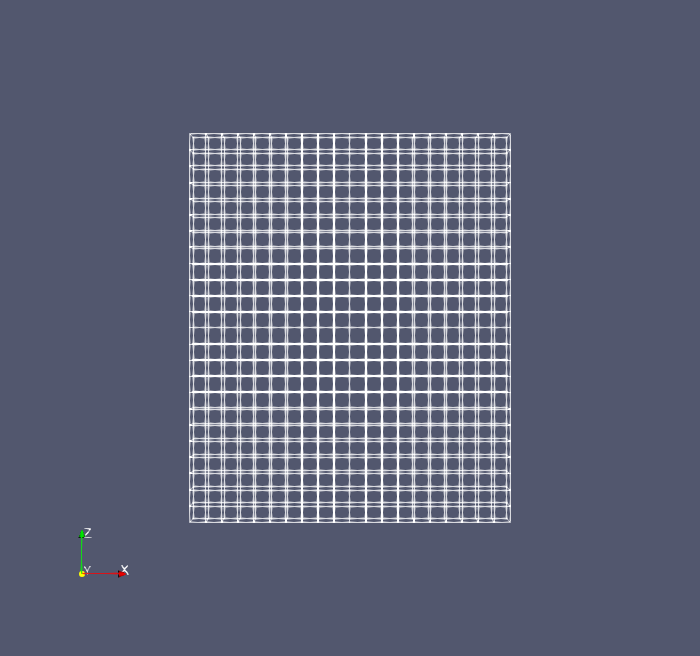
\includegraphics[width=.48\textwidth]{fig/pcl_mesh.png}\hfill
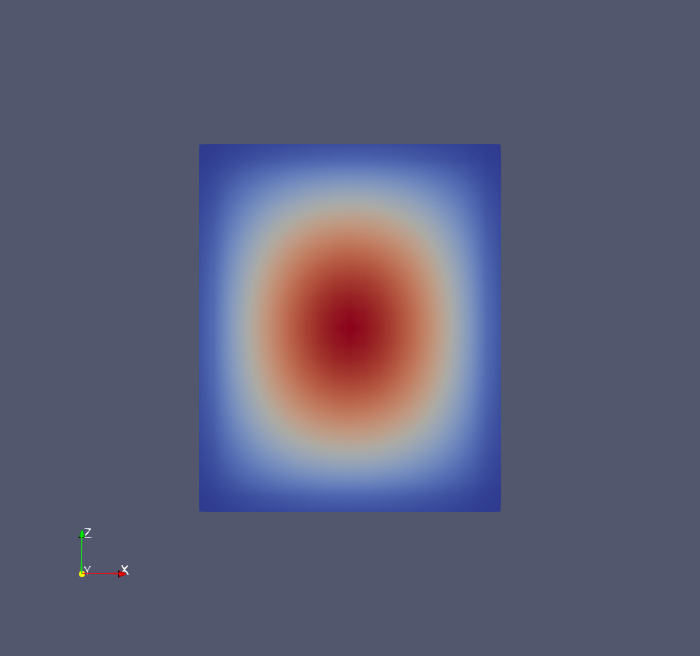
\includegraphics[width=.48\textwidth]{fig/pcl_steady_power.png}
\caption{pcL GeN-Foam computational mesh (left) and steady-state power density (right).}
\end{figure}

\begin{figure}[H]\centering
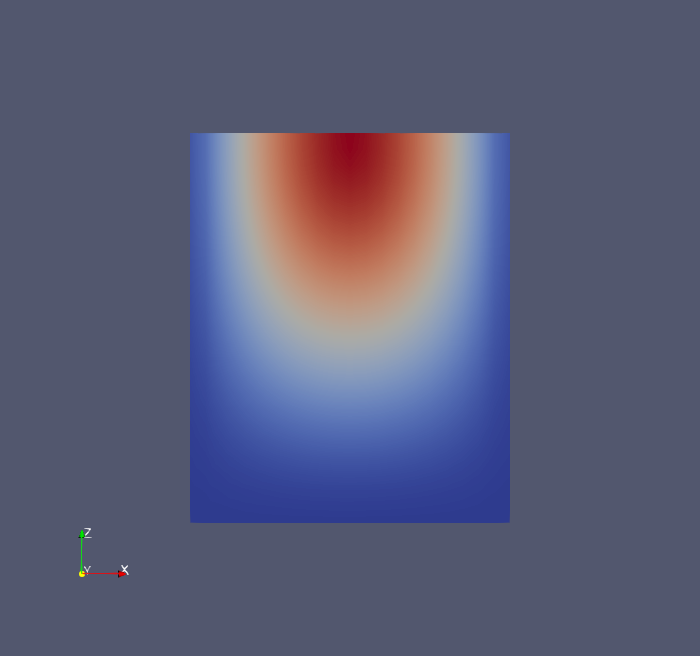
\includegraphics[width=.60\textwidth]{fig/pcl_steady_T.png}
\caption{pcL steady-state temperature field. The maximum lies in the upper portion of the
core, consistent with coolant heating as it rises through the channel.}
\end{figure}

\subsection{Reactivity insertion transient}
A $+0.5\,\$$ ramp ($0.00325\,\Delta k/k$) was inserted between $t=100$ and
$t=\SI{100.5}{\second}$.

\begin{figure}[H]\centering
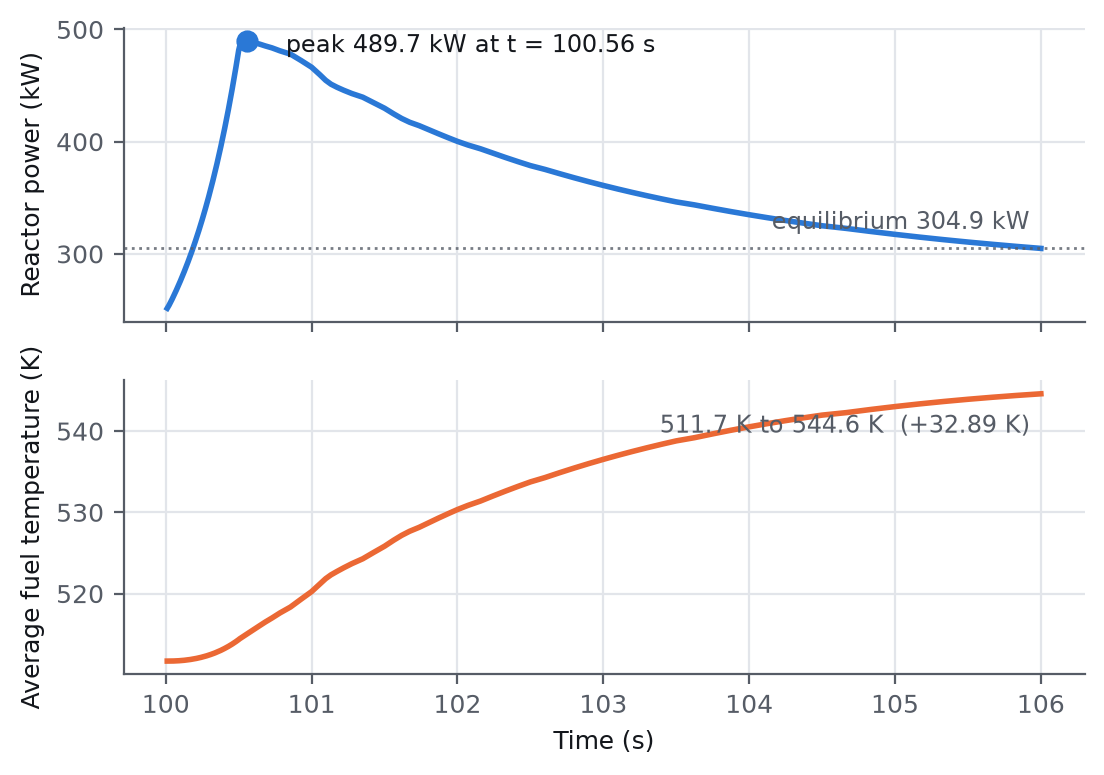
\includegraphics[width=\textwidth]{fig/pcl_transient.png}
\caption{pcL transient response. Power peaks at \SI{489.7}{\kilo\watt} and settles to a
Doppler-limited equilibrium of \SI{304.9}{\kilo\watt}; average fuel temperature rises
\SI{32.89}{\kelvin}.}
\end{figure}

\begin{table}[H]\centering\small
\caption{pcL transient summary.}
\begin{tabular}{@{}lrl@{}}
\toprule
\textbf{Quantity} & \textbf{Value} & \textbf{Note}\\
\midrule
Peak power & \SI{489723}{\watt} & at $t=\SI{100.56}{\second}$\\
Final power & \SI{304884}{\watt} & Doppler-limited equilibrium\\
Final average fuel $T$ & \SI{544.59}{\kelvin} & at $t=\SI{106}{\second}$\\
Net reactivity & $-3.87$\pcm & external $+325$ vs Doppler $-328.9$\\
\bottomrule
\end{tabular}
\end{table}

\begin{callout}{Feedback coefficient is an input, not a result}
The stated Doppler feedback of $-328.9$\pcm{} accompanies a fuel temperature rise from
511.70 to \SI{544.59}{\kelvin}, a span of \SI{32.89}{\kelvin}:
\[
\frac{-328.9\pcm}{\SI{32.89}{\kelvin}} = -10.000\ \mathrm{pcm/K}.
\]
The result is \emph{exactly} $-10.000$, which indicates a constant coefficient supplied as a
model input rather than one computed from nuclear data. Its origin is not documented in the
committed files. Section~\ref{sec:comp} compares it against pcM's computed value.
\end{callout}

\newpage
%======================================================================
\section{Results: pcM --- Cardinal / OpenMC / MOOSE / NekRS}
\subsection{Method}
Continuous-energy Monte Carlo neutronics (OpenMC) is coupled to finite-element heat
conduction (MOOSE) through Cardinal by Picard iteration: cell-averaged fission power is
transferred to the solid, and cell temperatures are returned to the neutronics. The coolant
is treated separately by spectral-element large-eddy simulation (NekRS).

Because the available hardware could not support a full-core coupled model, the coupled
calculation uses a \textbf{single-pin unit cell}. All coupled temperatures therefore
describe an \emph{average} pin.

\subsection{Neutronics}
\begin{table}[H]\centering\small
\caption{pcM eigenvalue results, ENDF/B-VIII.0, continuous-energy Monte Carlo.}
\begin{tabular}{@{}llrr@{}}
\toprule
\textbf{Quantity} & \textbf{Model} & \textbf{Value} & \textbf{Uncertainty}\\
\midrule
\kinf & 2-D unit cell, reflective & 1.384207 & $\pm\,21$\pcm\\
\keff & 3-D bare core, heterogeneous & 1.102059 & $\pm\,26$\pcm\\
\keff & 3-D bare core, homogenised & 1.145259 & $\pm\,74$\pcm\\
Leakage fraction & bare core & 0.20149 & $\pm\,0.00012$\\
Power peaking (max/avg) & 120 pins & 2.2544 & ---\\
Peak power density & bare core & \SI{6.595}{\watt\per\cubic\centi\meter} & ---\\
\bottomrule
\end{tabular}
\end{table}

The homogenised variant was computed specifically to separate geometry treatment from
solution method in the comparison of Section~\ref{sec:comp}. Its sensitivity to the
$S(\alpha,\beta)$ choice is itself notable: 1.145259 (H in H$_2$O), 1.132505 (H in ZrH) and
1.136651 (none) span 1275\pcm, more than twice the acceptance criterion.

\subsection{Fuel temperature coefficient}
The defining TRIGA parameter was computed from first principles by sweeping fuel temperature
with the moderator held at \SI{293}{\kelvin}, isolating fuel feedback.

\begin{figure}[H]\centering
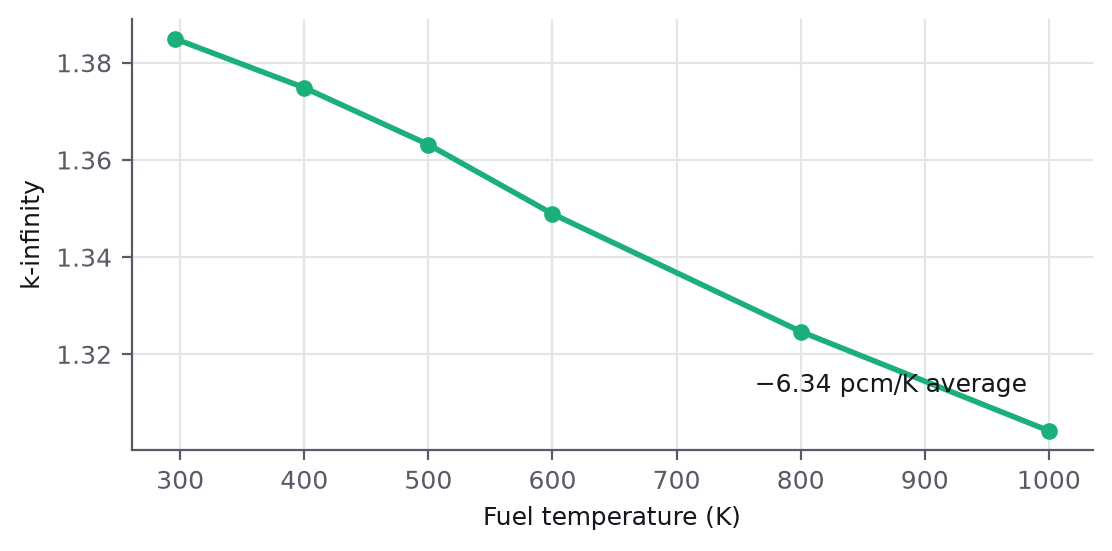
\includegraphics[width=.82\textwidth]{fig/fig4_tempcoeff.png}
\caption{pcM fuel temperature coefficient. $\kinf$ falls from 1.384926 at
\SI{296}{\kelvin} to 1.304249 at \SI{1000}{\kelvin}.}
\end{figure}

\begin{table}[H]\centering\small
\caption{pcM local fuel temperature coefficient by interval.}
\begin{tabular}{@{}lr@{}}
\toprule
\textbf{Band} & \textbf{Coefficient}\\
\midrule
296--\SI{400}{\kelvin} & $-5.08$\,pcm/K\\
400--\SI{500}{\kelvin} & $-6.24$\,pcm/K\\
\rowcolor{rowbg}500--\SI{600}{\kelvin} & $\mathbf{-7.76}$\,\textbf{pcm/K}\\
600--\SI{800}{\kelvin} & $-6.78$\,pcm/K\\
800--\SI{1000}{\kelvin} & $-5.92$\,pcm/K\\
\midrule
296--\SI{1000}{\kelvin} average & $-6.34$\,pcm/K\\
\bottomrule
\end{tabular}
\end{table}

The coefficient is large, negative, and becomes \emph{more} negative as the fuel heats. Both
features identify this as hydride physics rather than U-238 Doppler: a UO$_2$ LWR pin gives
roughly $-2$ to $-3$\,pcm/K and its magnitude does not grow in this way. The highlighted band
is the one in which pcL's transient operates.

\subsection{Coupled neutronics--conduction}
\begin{figure}[H]\centering
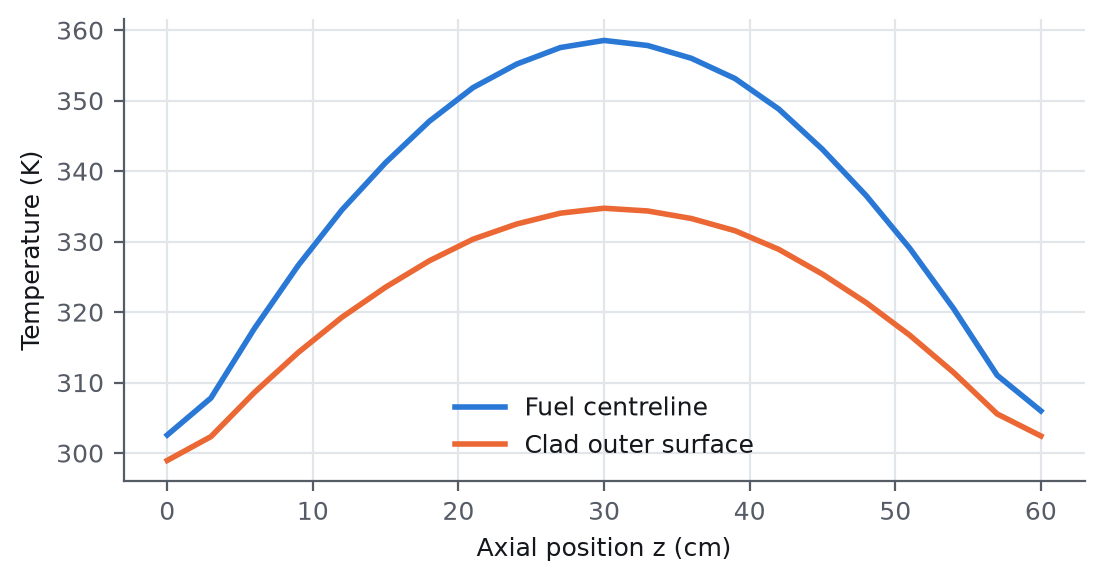
\includegraphics[width=.49\textwidth]{fig/fig1_axial.png}\hfill
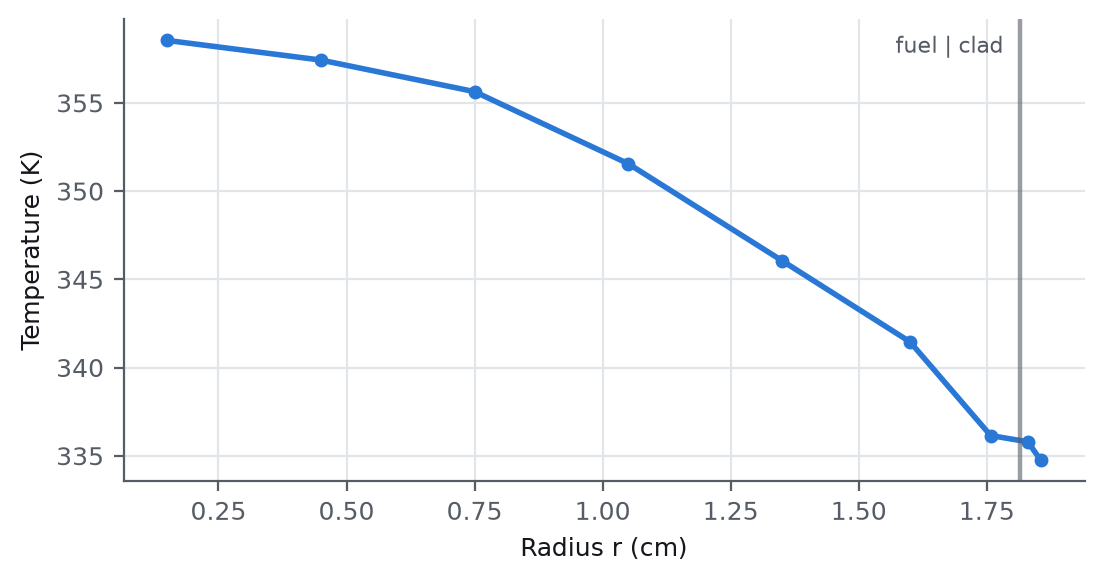
\includegraphics[width=.49\textwidth]{fig/fig2_radial.png}
\caption{pcM coupled temperature solution. Left: axial profile, slightly top-skewed
(\SI{305.98}{\kelvin} outlet against \SI{302.56}{\kelvin} inlet) because the coolant heats as
it rises. Right: radial profile at mid-plane; temperature is continuous across the
fuel--clad interface at \SI{1.815}{\centi\meter}, confirming the stitched contact.}
\end{figure}

\begin{table}[H]\centering\small
\caption{pcM coupled results and temperature drop budget.}
\begin{tabular}{@{}lrrr@{}}
\toprule
\textbf{Quantity} & \textbf{Value} & \textbf{Analytic} & \textbf{Share}\\
\midrule
Peak fuel temperature & \SI{359.0}{\kelvin} & \SI{362.8}{\kelvin} & ---\\
Peak clad temperature & \SI{336.2}{\kelvin} & --- & ---\\
Power integral & \SI{2083.33}{\watt} & \SI{2083.33}{\watt} & exact\\
\midrule
Film drop (clad $\rightarrow$ coolant) & \SI{40.3}{\kelvin} & \SI{42.4}{\kelvin} & 63\%\\
Fuel conduction drop & \SI{22.4}{\kelvin} & \SI{24.1}{\kelvin} & 35\%\\
Clad conduction drop & \SI{1.07}{\kelvin} & \SI{1.5}{\kelvin} & 2\%\\
\bottomrule
\end{tabular}
\end{table}

Agreement with the analytic cylindrical-conduction solution is within 1.1\%; the residual is
explained by the true axial power shape being flatter than the cosine the hand calculation
assumes. The film drop dominates and is the least certain term --- it derives from a
Dittus--Boelter correlation at $\mathrm{Re}=4755$, which is transitional and below the range
where that correlation is reliable.

\begin{figure}[H]\centering
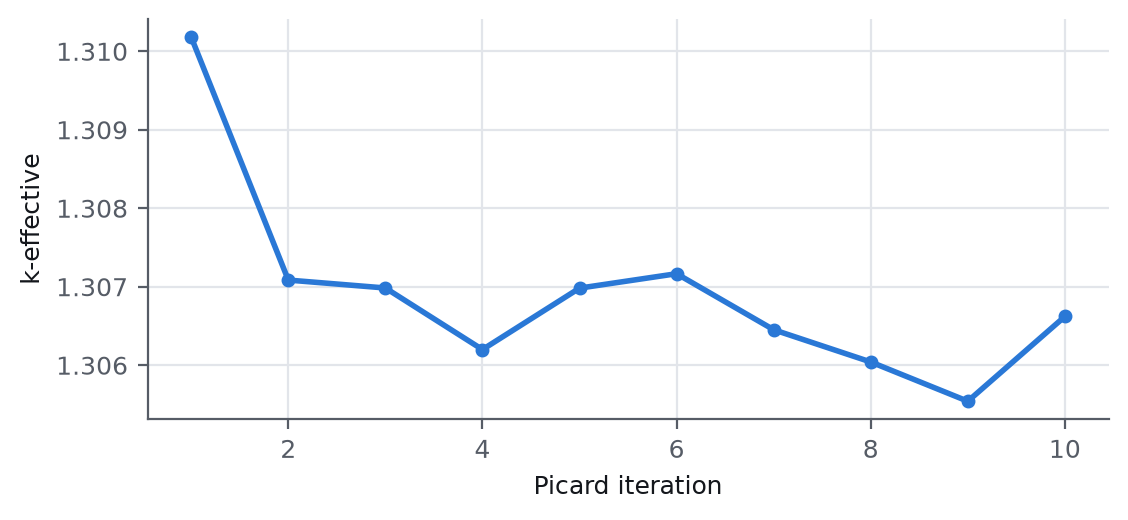
\includegraphics[width=.78\textwidth]{fig/fig3_picard.png}
\caption{pcM Picard convergence. $\keff$ settles within Monte Carlo noise after the first
temperature feedback; average fuel temperature is stable to \SI{e-8}{\kelvin}.}
\end{figure}

\subsection{Thermal-hydraulics}
An implicit large-eddy simulation of the coolant subchannel was run at $\mathrm{Re}=4755$,
polynomial order 7, 2880 spectral elements, on an NVIDIA GTX 1080~Ti. The run completed
20\,000 steps but covered only \textbf{1.17 flow-through times}.

\begin{figure}[H]\centering
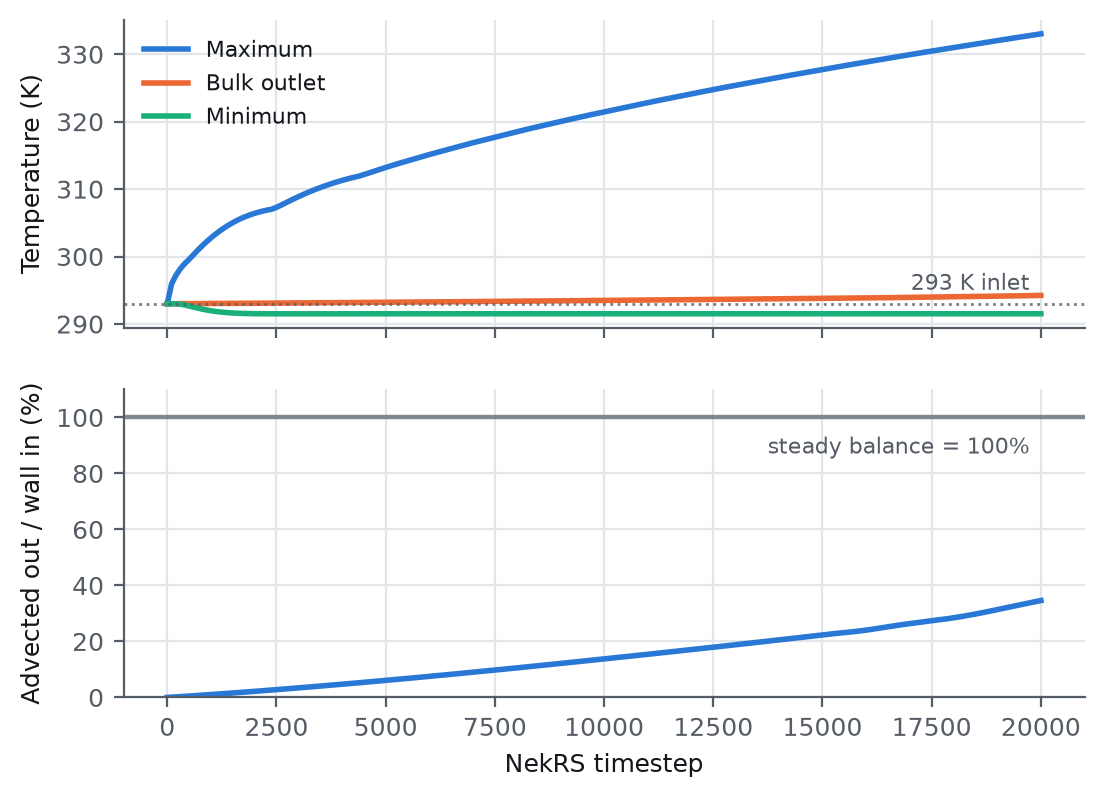
\includegraphics[width=.85\textwidth]{fig/fig7_nekrs.png}
\caption{pcM NekRS evolution. Upper: coolant temperatures, all still rising at the final
step, with the minimum below the \SI{293}{\kelvin} inlet throughout. Lower: energy closure
reaches only 34.6\% of the steady balance.}
\end{figure}

\begin{table}[H]\centering\small
\caption{pcM thermal-hydraulic state at 20\,000 steps.}
\begin{tabular}{@{}lrrl@{}}
\toprule
\textbf{Quantity} & \textbf{Value} & \textbf{Steady target} & \textbf{Status}\\
\midrule
Bulk outlet temperature & \SI{294.24}{\kelvin} & \SI{296.57}{\kelvin} & lower bound\\
Maximum temperature & \SI{333.03}{\kelvin} & --- & still rising\\
Minimum temperature & \SI{291.52}{\kelvin} & $\geq$ \SI{293}{\kelvin} & unphysical\\
Advected heat / wall heat & 34.6\% & 100\% & not closed\\
Mass-flow imbalance & 0.122\% & $\rightarrow 0$ & converged\\
\bottomrule
\end{tabular}
\end{table}

\begin{callout}[alertbg]{The pcM thermal-hydraulic field is not converged}
The flow field has converged --- mass imbalance is flat at 0.122\% from step 1400 onward ---
but only 34.6\% of the wall heat leaves the domain, so 65.4\% is still accumulating.
\textbf{The coolant temperatures above are lower bounds, not steady-state results.} Reaching
approximately five flow-throughs would require about 85\,700 steps and \SI{5.1}{\hour} of
GPU time.

A second defect is recorded rather than smoothed over: the minimum temperature lies below
the inlet in a domain whose only thermal boundary conditions are a \SI{293}{\kelvin} inlet
and a heated wall. With no heat sink this cannot be physical. It is an undershoot from the
high-pass filter stabilisation and it does not decay.
\end{callout}

\newpage
%======================================================================
\section{Comparison}\label{sec:comp}
\subsection{Overview}
\begin{table}[H]\centering\small
\caption{Case-by-case comparison. Only cases marked \emph{yes} support a direct numerical
difference; the acceptance criterion applies to those alone.}
\begin{tabular}{@{}clrrrl@{}}
\toprule
\textbf{\#} & \textbf{Case} & \textbf{pcL} & \textbf{pcM} & \textbf{Difference} & \textbf{Comparable}\\
\midrule
\rowcolor{rowbg}
1 & \kinf, unit cell & $1.388100$ & $1.384207$ & $-280$\pcm & yes\\
2 & \keff, heterogeneous & $1.240544$ & $1.102059$ & $+12566$\pcm & no --- method\\
3 & \keff, homogenised & $1.240544$ & $1.145259$ & $+8320$\pcm & partial\\
4 & Diffusion vs.\ Monte Carlo & $1.331$ & $1.388100$ & $-4114$\pcm & pcL-internal\\
5 & Fuel temp.\ coefficient & $-10.000$ & $-7.76$ & $-29\%$ & partial\\
6 & Power peaking & $2.45$ & $2.2544$ & $-8.0\%$ & no\\
7 & Max fuel temperature & \SI{594.2}{\kelvin} & \SI{359.0}{\kelvin} & $-\SI{235}{\kelvin}$ & no\\
8 & Max coolant temperature & \SI{306.5}{\kelvin} & \SI{294.2}{\kelvin} & --- & no\\
9 & Total power & \SI{250}{\kilo\watt} & \SI{250}{\kilo\watt} & $0$ & yes\\
10 & Transient peak power & \SI{489.7}{\kilo\watt} & not run & --- & no\\
11 & Two-group MGXS & full set & not generated & --- & no\\
12 & Solver acceptance & PASS & not recorded & --- & no\\
\bottomrule
\end{tabular}
\end{table}

\subsection{Case 1 --- the directly comparable quantity}
Both sides solved the same 2-D reflective pin cell with OpenMC continuous-energy Monte Carlo
and ENDF/B-VIII.0. This is the only case in which the two calculations solve the same
equations on the same geometry.

\begin{figure}[H]\centering
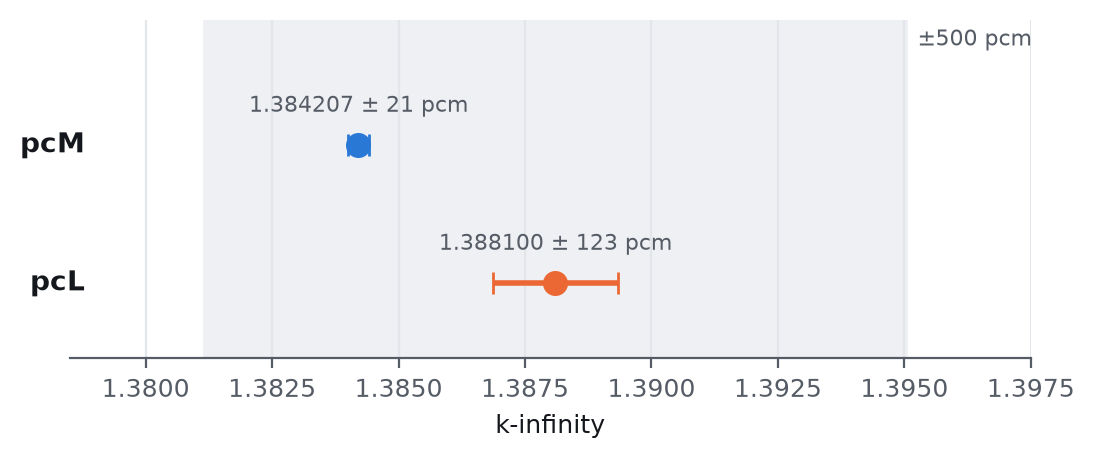
\includegraphics[width=.82\textwidth]{fig/fig5_kinf.png}
\caption{$\kinf$ comparison. Bars are $\pm 1\sigma$ counting statistics; the shaded band is
the 500\pcm{} acceptance criterion centred on pcL.}
\end{figure}

The difference is $\mathbf{-280}$\,\textbf{pcm} at $3.1\sigma$ --- statistically resolved but
comfortably inside the acceptance criterion. pcM's uncertainty is approximately six times
tighter, reflecting a 25-fold larger particle budget.

\emph{Interpretation.} Two independent implementations of the same specification, in the same
code, agree. This is the strongest evidence in the study that the shared problem definition
was interpreted consistently on both sides.

\subsection{Cases 2--4 --- the \keff{} difference is method, not error}
Both cores are bare boxes with vacuum boundaries: pcL's \texttt{validation\_step6.csv}
records the model verbatim as \emph{``eigenvalue diffusion, bare homogenized box vacuum
BCs''}. \textbf{Geometry is therefore not the explanation.} An earlier hypothesis that pcL
had modelled a graphite reflector is contradicted by this metadata and is withdrawn.

\begin{figure}[H]\centering
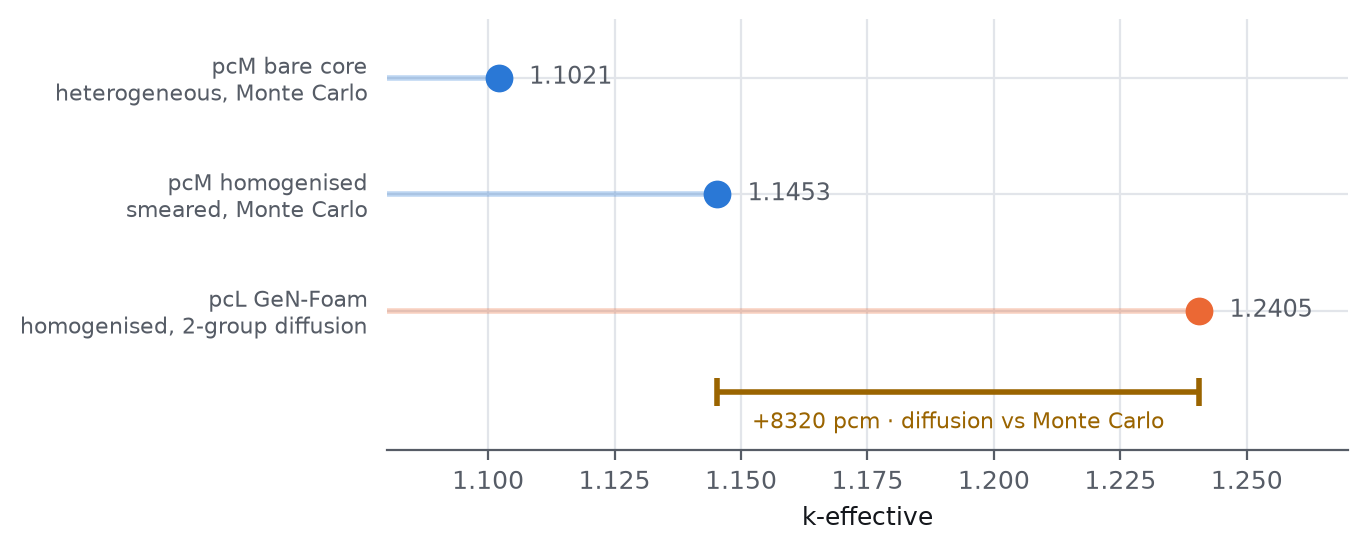
\includegraphics[width=.88\textwidth]{fig/fig6_keff.png}
\caption{Decomposition of the \keff{} difference into a homogenisation step (Monte Carlo on
both sides) and a solution-method step (same homogenised bare box).}
\end{figure}

\begin{table}[H]\centering\small
\caption{Two-step decomposition of the core eigenvalue difference.}
\begin{tabular}{@{}llrp{52mm}@{}}
\toprule
\textbf{Step} & \textbf{From $\rightarrow$ to} & \textbf{$\Delta\rho$} & \textbf{What it isolates}\\
\midrule
1. Homogenisation & pcM het.\ $\rightarrow$ pcM homog. & $+3920$\pcm & Monte Carlo both sides; pure geometry smearing\\
2. Solution method & pcM homog.\ $\rightarrow$ pcL & $+8320$\pcm & Same homogenised bare box; pure method\\
\midrule
\rowcolor{rowbg}
Total & pcM het.\ $\rightarrow$ pcL & $+12566$\pcm & ---\\
\bottomrule
\end{tabular}
\end{table}

The residual $+8320$\pcm{} is corroborated independently by pcL's own smoke test
(Case 4), which measures $-4114$\pcm{} between GeN-Foam diffusion and Monte Carlo on the pin
cell. The sign reverses between the two geometries --- diffusion under-predicts on the
reflective pin cell but over-predicts on the bare core --- which is consistent with leakage
treatment dominating in the bare case. pcM's core leaks 20.1\% of its neutrons, a regime in
which few-group diffusion theory is least reliable.

A further uncontrolled variable applies to Cases 2--3: the project workflow intended pcM to
generate the two-group MGXS and supply it to pcL, but \textbf{that phase was not run}. pcL
condensed its own constants independently (Case 11). Re-solving pcL's diffusion model with
pcM-generated cross sections would isolate the remaining method error cleanly.

\begin{callout}{The acceptance criterion does not apply across methods}
A 500\pcm{} threshold cannot meaningfully be applied between a continuous-energy Monte
Carlo eigenvalue and a two-group diffusion eigenvalue. They are different quantities, and
pcL's own data places the method difference at thousands of pcm on even the simplest
geometry. Applying the criterion across methods would manufacture a discrepancy that is not
evidence of error in either calculation.
\end{callout}

\subsection{Case 5 --- fuel temperature coefficient}
This is the most consequential physics difference, because the coefficient governs the entire
transient response.

\begin{table}[H]\centering\small
\caption{Fuel temperature coefficient, compared in pcL's own operating band.}
\begin{tabular}{@{}lll@{}}
\toprule
 & \textbf{Value} & \textbf{Origin}\\
\midrule
pcM, 500--\SI{600}{\kelvin} & $-7.76$\,pcm/K & computed from $S(\alpha,\beta)$ ZrH data\\
pcM, 296--\SI{1000}{\kelvin} average & $-6.34$\,pcm/K & computed\\
pcL, transient & $-10.000$\,pcm/K & constant input; origin undocumented\\
\midrule
\rowcolor{rowbg}
Difference in pcL's band & $-29\%$ & pcL more negative\\
\bottomrule
\end{tabular}
\end{table}

\begin{callout}[alertbg]{Recommended action}
A coefficient 29\% more negative shuts a power excursion down faster. pcL's peak power of
\SI{489.7}{\kilo\watt} is therefore plausibly \textbf{under-predicted}, and its equilibrium
reached sooner than a computed coefficient would give. For a TRIGA, where the prompt negative
coefficient \emph{is} the safety case, this warrants resolution.

pcM's value is traceable to a nuclear-data calculation; pcL's is not traceable from the
committed files. pcL should either substitute a temperature-dependent coefficient and re-run
the transient, or document the provenance of $-10$\,pcm/K.
\end{callout}

\subsection{Cases 6--8 --- thermal quantities}
These cannot be differenced as reported, for three independent reasons:
\begin{enumerate}\itemsep2pt
\item \textbf{pcM describes an average pin.} Its own peaking factor of 2.2544 implies a hot
channel is materially hotter, so the two fuel temperatures do not describe the same object.
\item \textbf{pcM's film coefficient is a correlation, not a solution.} Dittus--Boelter at
$\mathrm{Re}=4755$ supplies 63\% of pcM's total temperature rise, and is applied outside its
reliable range.
\item \textbf{pcM's coolant field is not converged} (34.6\% energy closure), so
\SI{294.2}{\kelvin} is a lower bound rather than a result.
\end{enumerate}

\subsection{Cases 10--12 --- no pcM counterpart}
The transient is out of pcM's defined scope: the project workflow specifies a steady-state
production run and defines no transient phase. This is a documented scope decision rather
than an omission, but it means pcL's transient results --- including the peak power on which
the safety argument rests --- have \textbf{no independent check}.

\newpage
%======================================================================
\section{Verification status}\label{sec:status}
\begin{callout}[alertbg]{This work is verified, not validated}
Verification asks whether the equations are solved correctly; validation asks whether the
equations describe reality, and is establishable only against experimental data.
\textbf{No experimental data was used in either calculation}, so no part of this study is
validated. Agreement between two codes is not a substitute --- two codes can agree and both
be wrong, particularly when they share a specification, a nuclear data library, or a
simplification. Here both share a bare-core model with no reflector and no control rods, so
\textbf{neither result describes a physical TRIGA at criticality}.
\end{callout}

\begin{table}[H]\centering\small
\caption{Verification status by level.}
\begin{tabular}{@{}llp{68mm}@{}}
\toprule
\textbf{Level} & \textbf{Status} & \textbf{Evidence}\\
\midrule
1. Software & MET & Both codes run to completion; pcL passes its reference cases; pcM conserves power exactly at \SI{2083.33}{\watt}\\
2. Numerical & PARTIAL & pcM neutronics and conduction converged; pcM CFD thermal field is not; no mesh or order refinement study either side\\
3. Physics & PARTIAL & pcM conduction within 1.1\% of analytic; ZrH feedback confirmed; but pcM CFD shows an unphysical sub-inlet temperature and pcL's feedback coefficient is an undocumented input\\
4. Cross-code & PARTIAL & Agreement to 280\pcm{} where methodologically comparable; larger differences decomposed and attributed to homogenisation and method\\
5. Experimental & NOT ATTEMPTED & No experimental data exists in this project\\
\bottomrule
\end{tabular}
\end{table}

\begin{table}[H]\centering\small
\caption{Actions required to close each gap, in priority order.}
\begin{tabular}{@{}rlp{58mm}l@{}}
\toprule
& \textbf{Gap} & \textbf{Action} & \textbf{Cost}\\
\midrule
1 & pcL feedback coefficient & Document or recompute the assumed $-10$\,pcm/K & ---\\
2 & \keff{} method gap & Generate pcM's two-group MGXS; re-solve pcL's diffusion with it & \SI{2}{\hour} CPU\\
3 & pcM CFD not converged & Extend to $\sim$5 flow-throughs after resolving the filter undershoot & \SI{5}{\hour} GPU\\
4 & pcM sub-inlet temperature & Reduce scalar HPFRT strength; verify with a short run & \SI{1}{\hour} GPU\\
5 & No mesh independence & Repeat at orders 5 and 8; compare integral quantities & \SI{8}{\hour} GPU\\
6 & pcM library deviation & Re-run coupled production on ENDF/B-VIII.0 & \SI{1}{\hour} CPU\\
7 & Reflector and rods & Agree whether they enter the benchmark & ---\\
8 & No validation & Obtain TRIGA experimental data & ---\\
\bottomrule
\end{tabular}
\end{table}

%======================================================================
\section{Conclusions}
\begin{enumerate}\itemsep4pt
\item \textbf{Where the two calculations are methodologically comparable, they agree.} The
Monte Carlo pin cell differs by 280\pcm{} at $3.1\sigma$, inside the
500\pcm{} acceptance criterion. This is the meaningful cross-code result of the study.

\item \textbf{The core eigenvalue difference is a method difference, not an error.} It
decomposes into 3920\pcm{} of homogenisation and 8320\pcm{} of
diffusion-versus-Monte-Carlo on geometrically identical bare cores. pcL's own data
independently measures a 4114\pcm{} method difference on the pin cell. Neither
calculation is thereby shown to be incorrect.

\item \textbf{The acceptance criterion is not transferable across methods.} A
500\pcm{} threshold between a Monte Carlo and a diffusion eigenvalue would
manufacture a false discrepancy.

\item \textbf{The fuel temperature coefficient is the outstanding physics question.} pcM
computes $-7.76$\,pcm/K in pcL's operating band from ZrH scattering data; pcL uses a constant
$-10.000$\,pcm/K of undocumented origin. Since this parameter governs the transient, and the
transient has no independent check, it is the highest-priority item.

\item \textbf{Two results are incomplete and are reported as such.} pcM's thermal-hydraulic
field has not converged, and pcM did not attempt the transient. Neither is presented as a
result.

\item \textbf{Neither calculation is validated.} Both cores are bare, without reflector or
control rods, and no experimental data was used. The study establishes cross-code
consistency where the methods permit it --- not fidelity to a physical reactor.
\end{enumerate}

\vspace{5mm}\hrule\vspace{2mm}
\footnotesize\color{ink2}
Data and inputs for both calculations:
\texttt{github.com/kavyawadhwa134/triga-markI-benchmark} (branch \texttt{master}).
pcM's full history and independence tag: \texttt{github.com/kavyawadhwa134/pcm-triga-cardinal}.
pcM results were frozen at tag \texttt{pcm-independent-v1} before any pcL file was read.
\end{document}
